\documentclass[12pt,titlepage]{article}
\usepackage[margin=1.25in]{geometry}
\usepackage{graphicx,amsmath,blindtext,minted}

%% Variables definition
\newcommand{\vSubject}{Object Oriented Programming}
\newcommand{\vSubtitle}{Class and Object}
\newcommand{\vName}{Muhammad Baihaqi Aulia Asy'ari}
\newcommand{\vNIM}{2241720145}
\newcommand{\vClass}{2I}
\newcommand{\vDepartment}{Information Technology}
\newcommand{\vStudyProgram}{D4 Informatics Engineering}

%% [START] Tikz related stuff
\usepackage{tikz}
\usetikzlibrary{svg.path,calc,shapes.geometric,shapes.misc}
\tikzstyle{terminator} = [rectangle, draw, text centered, rounded corners = 1em, minimum height=2em]
\tikzstyle{preparation} = [chamfered rectangle, chamfered rectangle sep=0.75em, draw, text centered, minimum height = 2em]
\tikzstyle{process} = [rectangle, draw, text centered, minimum height=2em]
\tikzstyle{decision} = [diamond, aspect=2, draw, text centered, minimum height=2em]
\tikzstyle{data}=[trapezium, draw, text centered, trapezium left angle=60, trapezium right angle=120, minimum height=2em]
\tikzstyle{connector} = [line width=0.25mm,->]
%% [END] Tikz related stuff

%% [START] Fancy header related stuff
\usepackage{fancyhdr}
\pagestyle{fancy}
\setlength{\headheight}{15pt} % compensate fancyhdr style
\fancyhead{}
\fancyfoot{}
\fancyfoot[L]{\thepage}
\fancyfoot[R]{\textit{\vSubject - \vSubtitle}}
\renewcommand{\footrulewidth}{0.4pt}% default is 0pt, overline for footer
%% [END] Fancy header related stuff

%% [START] Custom tabular command related stuff
\usepackage{tabularx}
\newcommand{\details}[2]{
    #1 & #2  \\
}
%% [END] Custom tabular command related stuff

%% [START] Figure related stuff
\newcommand{\image}[3][1]{
    \begin{figure}[h]
        \centering
        \includegraphics[#1]{#2}
        \caption{#3}
        \label{#3}
    \end{figure}
}
%% [END] Figure related stuff

%%
\usepackage{pgf-umlcd}

\renewcommand{\umldrawcolor}{black}
\renewcommand{\umlfillcolor}{white}
%%

%% [BEGIN] Custom enumerator
\usepackage{enumitem}
%% [END] Custom enumerator

%% [BEGIN] Paragraph indent
\usepackage{indentfirst}
%% [END] Paragraph indent

\begin{document}
\begin{titlepage}
    \centering
    \vfill
    {\bfseries\LARGE
        \vSubject\\
        \vskip0.25cm
        \vSubtitle
    }
    \vfill
    
\includegraphics[width=6cm]{images/polinema-logo.png}
    \vfill
    {
        \textbf{Name}\\
        \vName\\
        \vskip0.5cm
        \textbf{NIM}\\
        \vNIM\\
        \vskip0.5cm
        \textbf{Class}\\
        \vClass\\
        \vskip0.5cm
        \textbf{Department}\\
        \vDepartment\\
        \vskip0.5cm
        \textbf{Study Program}\\
        \vStudyProgram
    }
\end{titlepage}

\newpage

\setcounter{section}{3}

\section{Experiment}

\subsection{Experiment 1: Creating Class Diagram}
Case Study 2: \\

Dalam suatu perusahaan salah satu data yang diolah adalah data karyawan. Setiap karyawan memiliki id, nama, jenis kelamin, jabatan, jabatan, dan gaji. Setiap mahasiswa juga bisa menampilkan data diri pribadi dan melihat gajinya. \\

(In a company, one of the data processed is employee data. Each employee has an id, name, gender, job title, position, and salary. Each student can also display their personal data and see their salary.)

\begin{enumerate}
    \item Gambarkan desain class diagram dari studi kasus 1! \\ (Draw the class diagram of case study 1!)\\
    \texttt{Answer:} \\
    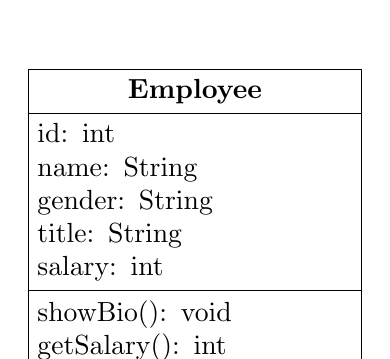
\begin{tikzpicture}
        \begin{class}[text width=4cm]{Employee}{0,0}
            \attribute{id: int}
            \attribute{name: String}
            \attribute{gender: String}
            \attribute{title: String}
            \attribute{salary: int}
            \operation{showBio(): void}
            \operation{getSalary(): int}
        \end{class}
    \end{tikzpicture}
    \item Sebutkan Class apa saja yang bisa dibuat dari studi kasus 1! \\ (Mention any classes that can be created from case study 1!) \\ \texttt{Answer:} The only class you can make in the study case is The Employee class
    \item Sebutkan atribut beserta tipe datanya yang dapat diidentifikasi dari masing-masing class dari studi kasus 1! \\ (List the attributes and their data types that can be identified from each of the class from case study 1!) \\
    \texttt{Answer:} 
    \begin{itemize}
        \item id : int
        \item name : String
        \item gender : String
        \item title : String
        \item salary : int
    \end{itemize}
    \item Sebutkan method-method yang sudah anda buat dari masing-masing class pada studi kasus 1! \\ (List the methods that you have created from each class in case study 1!) \\
    \texttt{Answer:} 
    \begin{itemize}
        \item showBio() : void
        \item getSalary() : int
    \end{itemize}
\end{enumerate}

\subsection{Experiment 2: Create and Access Class Component}
Case Study 2: \\

Perhatikan class diagram dibawah ini. Buatlah program berdasarkan class diagram tersebut! \\

(Take a look at the class diagram below. Create a program based on the class diagram!)

\begin{center}
    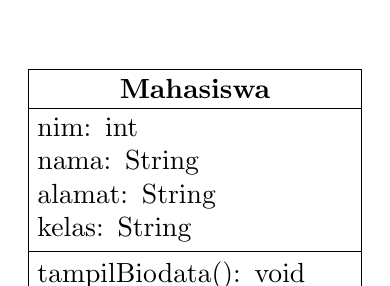
\begin{tikzpicture}
        \begin{class}[text width=4cm]{Mahasiswa}{0,0}
            \attribute{nim: int}
            \attribute{nama: String}
            \attribute{alamat: String}
            \attribute{kelas: String}
            \operation{tampilBiodata(): void}
        \end{class}
    \end{tikzpicture}
\end{center}

\subsubsection*{Steps}

\begin{enumerate}
    \item Bukalah text editor atau IDE, misalnya Notepad ++ / netbeans. - (Open a text editor or IDE, for example Notepad++ / netbeans.) \\
    \includegraphics[width=0.95\textwidth]{images/figures/fig1.png}
    \item Ketikkan kode program berikut ini: - (Type in the following program code:)
    \begin{minted}[autogobble,breaklines,linenos]{java}
        public class Mahasiswa {
            public int nim;
            public String nama;
            public String alamat;
            public String kelas;

            public void tampilBiodata() {
                System.out.println("Nim     : " + nim);
                System.out.println("Name    : " + nama);
                System.out.println("Alamat  : " + alamat);
                System.out.println("Kelas   : " + kelas);
            }
        }
    \end{minted}
    \item Simpan dengan nama file Mahasiswa.java. - (Save it with the filename Mahasiswa.java.)
    \item Untuk dapat mengakses anggota-anggota dari suatu obyek, maka harus dibuat instance dari class tersebut terlebih dahulu. Berikut ini adalah cara pengaksesan anggota- anggota dari class Mahasiswa dengan membuka file baru kemudian ketikkan kode program berikut: - (To be able to access the members of an object, an instance of the class must be created first. The following is how to access members of the Student class by opening a new file then typing the following program code:)
    \begin{minted}[autogobble,breaklines,linenos]{java}
        public class TestMahasiswa {
            public static void main(String[] args) {
                Mahasiswa mhs1 = new Mahasiswa();
                mhs1.nim = 101;
                mhs1.nama = "Lestari";
                mhs1.alamat = "Jl. Vinolia No 1A";
                mhs1.kelas = "1A";
                mhs1.tampilBiodata();
            }
        }
    \end{minted}
    \item Simpan file dengan TestMahasiswa.java - (Save the file as TestMahasiswa.java)
    \item Jalankan class TestMahasiswa - (Run the TestMahasiswa class)
    \begin{minted}[autogobble,breaklines,linenos]{text}
        PS D:\Kuliah>  d:; cd 'd:\Kuliah'; & 'C:\Program Files\Java\jdk-18.0.2.1\bin\java.exe' '-XX:+ShowCodeDetailsInExceptionMessages' '-cp' 'C:\Users\G4CE-PC\AppData\Roaming\Code\User\ workspaceStorage\80d97a47d24665dc0bce7ab1e048ecbd\ redhat.java\jdt_ws\Kuliah_28156aa7\bin' 'Experiment2.TestMahasiswa'
        Nim     : 101
        Name    : Lestari
        Alamat  : Jl. Vinolia No 1A
        Kelas   : 1A
    \end{minted}
    \item Jelaskan pada bagian mana proses pendeklarasian atribut pada program diatas! - (Explain which part of the attribute declaration process in the program above!) \\
    \texttt{Answer:} attribute declaration happends in line 2 until line 5 in Mahasiswa Class
    \item Jelaskan pada bagian mana proses pendeklarasian method pada program diatas! - (Explain which part of the method declaration process in the program above!) \\
    \texttt{Answer:} method declaration happends in line 7 until line 12 in Mahasiswa Class
    \item Berapa banyak objek yang di instansiasi pada program diatas! - (How many objects are instantiated in the above program!) \\
    \texttt{Answer:} Only one object instantiated in the TestMahasiswa Class.
    \item Apakah yang sebenarnya dilakukan pada sintaks program “mhs1.nim=101” ? - (What does the program syntax "mhs1.nim=101" actually do?) \\
    \texttt{Answer:} it instantiate a value to one of the mhs1's attribute
    \item Apakah yang sebenarnya dilakukan pada sintaks program “mhs1.tampilBiodata()” ? - (What does the syntax of the program "mhs1.tampilBiodata()" actually do?) \\
    \texttt{Answer:} it calls a function that the mhs1 has, it is used to print the bio of the mhs1.
    \item Instansiasi 2 objek lagi pada program diatas! - (Instantiate 2 more objects in the program above!)
    \begin{minted}[autogobble,breaklines,linenos]{java}
        public class TestMahasiswa {
            public static void main(String[] args) {
                Mahasiswa mhs1 = new Mahasiswa();
                mhs1.nim = 101;
                mhs1.nama = "Lestari";
                mhs1.alamat = "Jl. Vinolia No 1A";
                mhs1.kelas = "1A";
                mhs1.tampilBiodata();

                Mahasiswa mhs2 = new Mahasiswa();
                Mahasiswa mhs3 = new Mahasiswa();
            }
        }
    \end{minted}
\end{enumerate}

\subsection{Experiment 3: Create Methods with Arguments/Parameters and Returns}
\subsubsection*{Steps}
\begin{enumerate}
    \item Bukalah text editor atau IDE, misalnya Notepad ++ / netbeans. - (Open a text editor or IDE, for example Notepad++ / netbeans.)
    \item Ketikkan kode program berikut ini: - (Type in the following program code:)
    \begin{minted}[autogobble,breaklines,linenos]{java}
        public class Barang {
            public String namaBrg;
            public String jenisBrg;
            public int stok;

            public void tampilBarang() {
                System.out.println("Nama Barang     : " + namaBrg);
                System.out.println("Jenis Barang    : " + jenisBrg);
                System.out.println("Stok            : " + stok);
            }

            public int tambahStok(int brgMasuk) {
                int stokBaru = brgMasuk+stok;
                return stokBaru;
            }
        }
    \end{minted}
    \item Simpan dengan nama file Barang.java - (Save it with the file name Barang.java)
    \item Untuk dapat mengakses anggota-anggota dari suatu obyek, maka harus dibuat instance dari class tersebut terlebih dahulu. Berikut ini adalah cara pengaksesan anggota-anggota dari class Barang dengan membuka file baru kemudian ketikkan kode program berikut: - (To be able to access the members of an object, an instance of the class must be created first. The following is how to access the members of the Goods class by opening a new file then typing the following program code:)
    \begin{minted}[autogobble,breaklines,linenos]{java}
        public class TestBarang {
            public static void main(String[] args) {
                Barang brg1 = new Barang();
                brg1.namaBrg = "Pensil";
                brg1.jenisBrg = "ATK";
                brg1.stok = 10;
                brg1.tampilBarang();

                System.out.println("Stok baru adalah " + brg1.tambahStok(20));
            }
        }
    \end{minted}
    \item Simpan dengan nama file TestBarang.java - (Save it with the file name TestBarang.java)
    \item Jalankan program tersebut! - (Run the program!)
    \item Apakah fungsi argumen dalam suatu method? - (What is the function of arguments in a method?) \\
    \texttt{Answer:} it is used as a variable input to be used inside the methods
    \item Ambil kesimpulan tentang kegunaan dari kata kunci return , dan kapan suatu method harus memiliki return! - (Draw conclusions about the use of the return keyword, and when a method should have a return!) \\
    \texttt{Answer:} return is used to give a value when a method is called. the return keyword is used when a method data type is not void.
\end{enumerate}

\subsection{Assignment}

\begin{enumerate}
    \item Suatu toko persewaan video game salah satu yang diolah adalah peminjaman, dimana data yang dicatat ketika ada orang yang melakukan peminjaman adalah id, nama member, nama game, dan harga yang harus dibayar. Setiap peminjaman bisa menampilkan data hasil peminjaman dan harga yang harus dibayar. Buatlah class diagram pada studi kasus diatas! - (One of the video game rental shops that is processed is borrowing, where the data recorded when someone borrows is the id, member name, game name, and price to be paid. Each loan can display the loan result data and the price to be paid. Draw a class diagram for the case study above!) \\\\
    Penjelasan: -(Explanation: )
    \begin{itemize}
        \item Harga yang harus dibayar diperoleh dari lama sewa x harga. - (The price to be paid is obtained from the length of the lease x the price.)
        \item Diasumsikan 1x transaksi peminjaman game yang dipinjam hanya 1 game saja. - (It is assumed that 1x game loan transaction is borrowed only 1 game.)
    \end{itemize}
    \texttt{Answer: }\\\\
    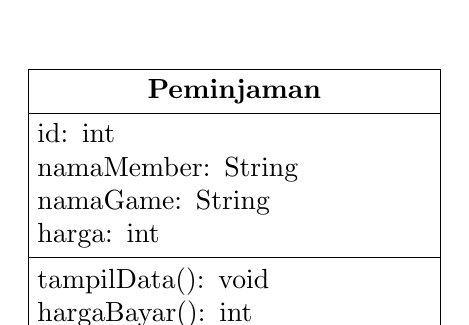
\begin{tikzpicture}
        \begin{class}[text width=5cm]{Peminjaman}{0,0}
            \attribute{id: int}
            \attribute{namaMember: String}
            \attribute{namaGame: String}
            \attribute{harga: int}
            \operation{tampilData(): void}
            \operation{hargaBayar(): int}
        \end{class}
    \end{tikzpicture}
    \item Buatlah program dari class diagram yang sudah anda buat di no 1! - (Create a program from the class diagram that you have created in number 1!)
    \begin{minted}[autogobble,breaklines,linenos]{java}
        public class Peminjaman {
            public int id;
            public String namaMember;
            public String namaGame;
            public int harga;

            public void tampilData() {
                System.out.println("ID Transaksi: " + id);
                System.out.println("Nama Member : " + namaMember);
                System.out.println("Nama Game   : " + namaGame);
                System.out.println("Harga Game  : " + harga);
            }

            public int hargaBayar(int lamaSewa) {
                return lamaSewa * lamaSewa;
            }
        }
    \end{minted}
    \includegraphics[width=0.9\textwidth]{images/figures/fig2.png}
    \item Buatlah program sesuai dengan class diagram berikut ini: - (Create a program according to the following class diagram:)\\
    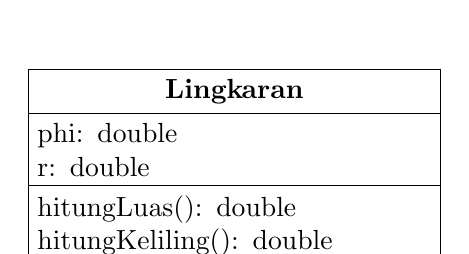
\begin{tikzpicture}
        \begin{class}[text width=5cm]{Lingkaran}{0,0}
            \attribute{phi: double}
            \attribute{r: double}
            \operation{hitungLuas(): double}
            \operation{hitungKeliling(): double}
        \end{class}
    \end{tikzpicture}
    \begin{minted}[autogobble,breaklines,linenos]{java}
        public class Lingkaran {
            public double phi = 3.141592;
            public double r;

            public double hitungLuas() {
                return phi * r * r;
            }

            public double hitungKeliling() {
                return 2 * phi * r;
            }
        }
    \end{minted}
    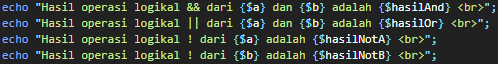
\includegraphics[width=0.9\textwidth]{images/figures/fig3.png}
    \item Buatlah program sesuai dengan class diagram berikut ini: - (Create a program according to the following class diagram:)\\
    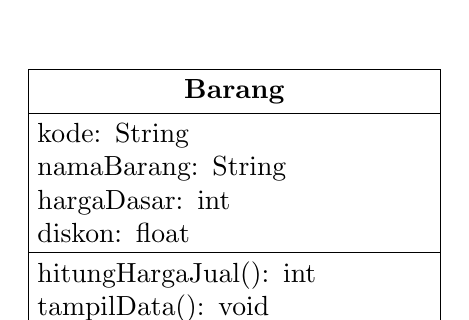
\begin{tikzpicture}
        \begin{class}[text width=5cm]{Barang}{0,0}
            \attribute{kode: String}
            \attribute{namaBarang: String}
            \attribute{hargaDasar: int}
            \attribute{diskon: float}
            \operation{hitungHargaJual(): int}
            \operation{tampilData(): void}
        \end{class}
    \end{tikzpicture}
    \\ Deskripsi / Penjelasan : - (Description / Explanation :)
    \begin{itemize}
        \item Nilai atribut hargaDasar dalam Rupiah dan atribut diskon dalam \% - (The value of the hargaDasar attribute in Rupiah and the diskon attribute in \%)
        \item Method hitungHargaJual() digunakan untuk menghitung harga jual dengan perhitungan berikut ini: \\ - (The calculateSalePrice() method is used to calculate the sale price with the following calculation:) \\ \textbf{harga jual = harga dasar – (diskon x harga dasar)}
        \item Method tampilData() digunakan untuk menampilkan nilai dari kode, namaBarang, hargaDasar, diskon dan harga jual. - (The tampilData() method is used to display the values of kode, namaBarang, hargaDasar, diskon and harga jual.)
    \end{itemize}
    \begin{minted}[autogobble,breaklines,linenos]{java}
        public class Barang {
            public String kode;
            public String namaBarang;
            public int hargaDasar;
            public float diskon;

            public int hitungHargaJual() {
                return hargaDasar - ((int) (diskon * hargaDasar));
            }

            public void tampilData() {
                System.out.println("Kode Barang : " + kode);
                System.out.println("Nama Barang : " + namaBarang);
                System.out.println("Harga Barang: Rp" + hargaDasar);
                System.out.println("Diskon      : " + diskon + "%");
                System.out.println("Harga Jual  : Rp" + hitungHargaJual());
            }
        }
    \end{minted}
    \includegraphics[width=0.9\textwidth]{images/figures/fig4.png}
\end{enumerate}

\end{document}